Resumen de diferentes partes: 

- Qué son los agentes, cómo interactúan con las herramientas y qué abstracciones ofrecen los frameworks que comentamos
- Ajuste de agentes -> LoRa?
- El protocolo MCP
- El estado del arte en arquitecturas de agentes LLM y sistemas RAG
- El estado del arte en agentes integrados a proyectos software

2. Agentes LLM (Fundamentos y funcionamiento básico)

¿Qué son los agentes LLM?
2.1. Modelos LLM
2.2. Interacción con herramientas
2.3. Abstracciones en frameworks

\section{Agentes LLM}

Los agentes de Inteligencia Artificial son programas informáticos que implementan modelos computaciones avanzados para ejecutar diversas funciones específicas del contexto en el que se aplican. Tras aproximadamente siete décadas y media de investigación, los esfuerzos en el campo se han focalizado en agentes basados en Grandes Modelos de Lenguaje (LLM). 

\subsection{Modelos LLM}

Los modelos de lenguaje (LM) constituyen sistemas de inteligencia artificial especializados en el procesamiento del lenguaje natural. Entre estos, destacan los grandes modelos de lenguaje, diseñados para acometer tareas  como la clasificación y generación de contenido lingüístico. Su fundamento técnico reside en las redes neuronales que implementan la arquitectura Transformer [Attention is All You Need]. Para comprender el funcionamiento de dicha arquitectura, resulta imprescindible asimilar previamente conceptos como la tokenización y las representaciones vectoriales del lenguaje.

\paragraph{Tokens}
Los tokens son las unidades mínimas de texto que el modelo procesa. Al ser modelos computacionales, la única representación que entienden son matrices. Para representar el lenguaje en forma matricial, es necesario dividir el texto en unidades mínimas. Estos pueden ser carácteres, segmentos de texto, palabras, etc. El conjunto de tokens que el modelo puede interpretar se conoce como vocabulario. De esta forma, el modelo puede representar el texto como una matriz de tokens, donde cada token es representado por un vector numérico conocido como one-hot encoding. Este vector tiene un valor de 1 en la posición del token y 0 en el resto de posiciones para el vocabulario.

\paragraph{Representaciones vectoriales}
Más conocidos como embeddings, son vectores numéricos de tamaño fijo los cuales representan la semántica de un token. Su alta dimensionalidad les permite capturar la semántica del texto de forma profunda. Pueden contener desde 768 dimensiones en modelos como BERT-base hasta más de 16 mil dimensiones en modelos del estado del arte. Las representaciones son aprendidas durante el entrenamiento del modelo, por ejemplo, una dimensión podría aprender a representar conceptos como la abstracción de la palabra. En este caso, la representación del token ``animal`` tendría un valor superior en esta dimensión que la representación de la palabra ``gato``.

A grandes rasgos, esta arquitectura utiliza el concepto de ``atención`` para enriquecer la comprensión que el modelo tiene sobre el texto. Para ello, el modelo primero transforma la respresentación de las palabras de entrada para que estas contengan información sobre el contexto de las demás palabras. Esto se consigue aplicando varias capas de atención, las cuales consisten en una serie de operaciones matriciales las cuales transfieren semántica entre las palabras. Tras obtener una representación enriquecida de las palabras, los modelos pueden realizar tareas como la generación, clasificación, traducción, etc.

Los agentes LLM utilizan en su mayoría modelos decodificadores autorregresivos, como GPT, Claude-Sonnet o Llama. Estos son un tipo de transformer focalizados en la generación de texto. Optimizados para la generación autorregresiva, la atención de cada token es sólo aplicada sobre los tokens anteriores. Esto permite que el modelo sólo calcule la atención que tokens anteriores aplican sobre el token actual, sin modificar la reresentación de los anteriores. 

La figura \ref{fig:atencion_gato} muestra un ejemplo simplificado del cómputo de atención para la frase ``El gato duerme``. Para generar la siguiente palabra, el modelo atenderá con diferentes magnitudes a la secuencia previa. En este caso, el modelo prestará más atención al hecho de que el gato esté durmiendo que al color del gato, por lo que la palabra  ``duerme`` tendrá más relevancia que la palabra ``negro`` a la hora de definir la semántica de la siguiente palabra. De esta forma, se calculará la probabilidad de la siguiente palabra teniendo en cuenta todo el vocabulario. De la misma forma, el modelo aplicó la influencia de las palabra ``El`` y ``gato`` para generar la palabra negro, pero no se le aplicará a la palabra ``gato`` la influencia de la palabra ``negro``.

\begin{figure}
    \centering
    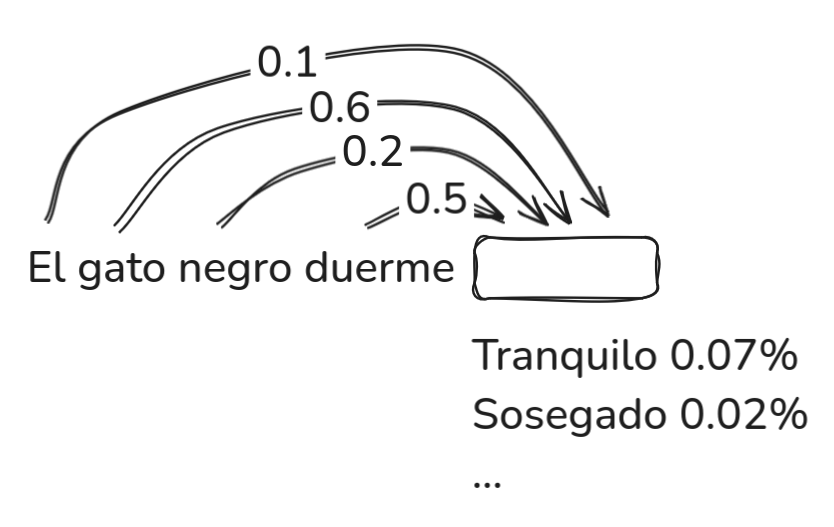
\includegraphics[width=0.65\linewidth]{figures/atencion_poc.png}
    \caption{Ejemplo simplificado de cómputo de atención para la frase \textquotedbl El gato duerme\textquotedbl}
    \label{fig:atencion_gato}
\end{figure}

En implementaciones reales, la atención aplicada desde un token origen hacia un token destino se calcula mediante operaciones matriciales con las representaciones vectoriales del ambos tokens y las matrices de atención, las cuales son parte de los pesos del modelo. Por ejemplo, al entrenar el modelo una de estas matrices podría aprender a extraer la connotación negativa que el token origen aplica al token destino. 

\subsection{Interacción con herramientas}

\subsection{Abstraciones en frameworks}










